\documentclass[bachelor, och, referat, times]{SCWorks}
% параметр - тип обучения - одно из значений:
%    spec     - специальность
%    bachelor - бакалавриат (по умолчанию)
%    master   - магистратура
% параметр - форма обучения - одно из значений:
%    och   - очное (по умолчанию)
%    zaoch - заочное
% параметр - тип работы - одно из значений:
%    referat    - реферат
%    coursework - курсовая работа (по умолчанию)
%    diploma    - дипломная работа
%    pract      - отчет по практике
%    pract      - отчет о научно-исследовательской работе
%    autoref    - автореферат выпускной работы
%    assignment - задание на выпускную квалификационную работу
%    review     - отзыв руководителя
%    critique   - рецензия на выпускную работу
% параметр - включение шрифта
%    times    - включение шрифта Times New Roman (если установлен)
%               по умолчанию выключен 

\usepackage[T2A]{fontenc}
\usepackage[utf8]{inputenc}
\usepackage{graphicx}
\usepackage[sort,compress]{cite}
\usepackage{amsmath}
\usepackage{amssymb}
\usepackage{amsthm}
\usepackage{fancyvrb}
\usepackage{longtable}
\usepackage{array}
\usepackage{makecell}
\usepackage{multirow}
\usepackage[english,russian]{babel}

\usepackage{tempora}
\usepackage[hidelinks]{hyperref}

\usepackage{pgfplots}
\usepackage{tikz}
\usepackage{float}
\pgfplotsset{compat = newest}

\usepackage{minted}
\setminted[c++]{linenos, breaklines = true, style = bw, fontsize = \small}

\newcommand{\eqdef}{\stackrel {\rm def}{=}}

\newtheorem{lem}{Лемма}

\begin{document}


% Кафедра (в родительном падеже)
\chair{математической кибернетики и компьютерных наук}

% Тема работы
\title{Отчетная работа}

% Курс
\course{1}

% Группа
\group{151}

% Факультет (в родительном падеже) (по умолчанию "факультета КНиИТ")
%\department{факультета КНиИТ}

% Специальность/направление код - наименование

\napravlenie{09.03.04 "--- Программная инженерия}

% Фамилия, имя, отчество в родительном падеже
\author{Смирнова Егора Ильича}

% Год выполнения отчета
\date{2023}

\maketitle

% Включение нумерации рисунков, формул и таблиц по разделам
% (по умолчанию - нумерация сквозная)
% (допускается оба вида нумерации)
%\secNumbering

\tableofcontents

% Раздел "Обозначения и сокращения". Может отсутствовать в работе
%\abbreviations
%\begin{description}
%    \item $|A|$  "--- количество элементов в конечном множестве $A$;
%    \item $\det B$  "--- определитель матрицы $B$;
%    \item ИНС "--- Искусственная нейронная сеть;
%    \item FANN "--- Feedforward Artifitial Neural Network
%\end{description}

% Раздел "Определения". Может отсутствовать в работе
%\definitions

% Раздел "Определения, обозначения и сокращения". Может отсутствовать в работе.
% Если присутствует, то заменяет собой разделы "Обозначения и сокращения" и "Определения"
%\defabbr


% Раздел "Введение"
\intro

Тут будет объяснение что как

\section{Лабораторная работа <<Поверхностное натяжение>>}
\textbf{Цель работы:} определение коэффициента поверхностного натяжения методом <<Разрыва тонкого слоя жидкости>>.

\textbf{Принадлежности:} кольцо для изучения поврхностного натяжения, точный динамометр $(0.1H)$, стакан из комплекта дополнительного оборудования, лабораторный подъёмный столик со штативом из нержавеющей стали и крючком, штангенциркуль.Установка (рис.\ref{fig:installation})

\begin{figure}[!h]
    \centering
    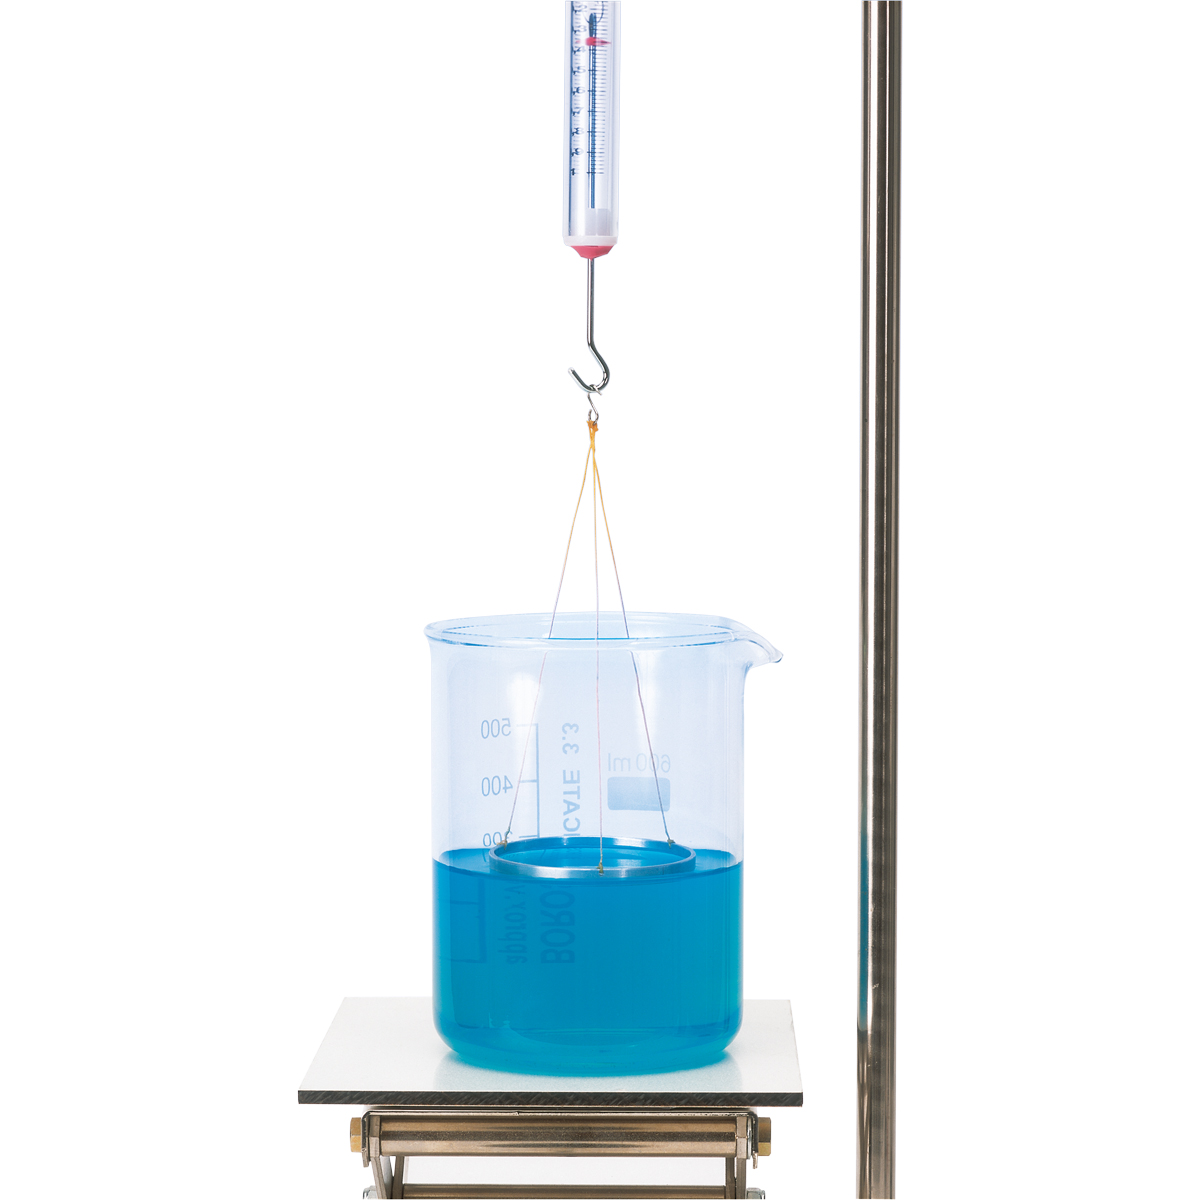
\includegraphics[width = 0.5\textwidth]{image/image.png}
    \caption{установка}
    \label{fig:installation}
\end{figure}

\textbf{Вывод рабочей формулы:}

Поверхностное натяжение жидкости "--- это её свойство на границе контакта с окружающей средой. Оно обусловлено тем, что молекула жидкости, находящаяся на её поверхности, испытывает действие сил со стороны соседних с ней молекул жидкости только из половины пространства, ограниченной поверхностью этой жидкости, в то время как молекула внутри жидкости испытывает воздействие со всех сторон. Поэтому молекула в поверхностном слое испытывает воздействие результирующей силы, направленной перпендикулярно к поверхности внутрь жидкости.

Действие этой силы приводит к сокращению площади поверхности жидкости. Взаимодействие молекул в поверхностном слое также обуславливает наличие горизонтальной составляющей сил, способствующей стремлению площади поверхности к сокращению. Эти силы получили название сил поверхностного натяжения. Сила поверхностного \texttt{$F_\text{н}$} натяжения направлена по касательной к поверхности жидкости. За счёт воздействия сил поверхностного натяжения молекулы жидкости в поверхностном слое обладаююь дополнительной потенциальной энергией по сравнению с молекулами внутреннего объема. Это дополнительная энергия называется поверхностной энергией \texttt{$W_\text{пов}$} и пропорциональна площади поверхности жидкости:

\begin{equation*}
    W_\text{пов} = \alpha S
\end{equation*}

Коэффициент пропорциональности \texttt{$\alpha$} является мерой свободной поверхности.

\begin{equation*}
    \alpha = \frac{W_\text{пов}}{S}
\end{equation*}

называется коэффициентом поврхностного натяжения и зависит от природы и состояния как жидкости, так и той среды с которой соприкасается её поверхность. То есть от физико"=химических свойств, определяющих энергию взаимодействия их молекул.

Физический смысл коэффициента поверхностного натяжения состоит в том, что он численно равен рабооте, затрачиваемой на образование $1 \text{м}^2$ поверхности жидкости при постоянной температуре.

\begin{equation*}
    \alpha = \frac{d A_\text{пов}}{d S}
\end{equation*}

и представляет собой силу сцепления поверхностной плёнки жидкости. Вызванную взаимным притяжением молекул, находящихся по обе стороны линии контура её разрыва, дейстующую на единицу длины:

\begin{equation*}
    F_\text{н} = \alpha L
\end{equation*}

Определить коэффициент поверхностного натяжения можно увеличив поверхность жидкости на величину \texttt{$d S$} переводом в поверхностный слой некоторого числа молекул, совершив тем самым работы \texttt{$d A_\text{пов}$}. Осуществить это возможно при помощи кольца с острой кромкой, которое изначально полностью погружено в жидкость. Если, приложив внешнюю силу \texttt{$F_\text{вн}$}, компенсирующую силу поверхностного натяжения \texttt{$F_\text{вн}$}, кольцо медленно извлеать из жидкости, тонкий слой жидкости вытягивается вверх за его нижним краем (рис. \ref{fig:installation})

\begin{equation*}
    d A_\text{пов} = F_\text{вн} \Delta x
\end{equation*}

Когда кольцо поднимается на высоту \texttt{$\Delta x$}, площадь поверхности тонкого слоя увеличивается снаружи и внутри кольца в общем на:

\begin{equation*}
    d S = 4 \pi R \Delta x
\end{equation*}

где \texttt{$R$}"--- радиус кольца. 

Если сила \texttt{$F_\text{вн}$}, прилагаемая при подъёме кольца, превышает \texttt{$F_\text{н}$}, тонкий слой жидкости рвется. В этот момент можно определить:

\begin{equation}
    \alpha = \frac{F_\text{вн}}{4 \pi R}
\end{equation}

\vspace{0.5cm}

\textbf{Описание установки:}

В этой работе металлическое кольцо с острой нижней кромкой свисает в горизонтальном положении с точного динамометра. Сначала кольцо полностью погружено в испытываемую жидкость (например, в воду), затем оно медленно извлекается из жидкости. Тонкий слой жидкости разрывается, когда сила вытягивания \texttt{$F_\text{вн}$}, превышает предельное значение \texttt{$F_\text{н}$}.

\vspace{0.5cm}

\textbf{Порядок выполнения работы:}
\begin{enumerate}
    \item {Установить лабораторный подъёмный столик на минимальный уровень подъёма.}
    \item {Подвесить динамометр на вертикальный штатив с крючком.}
    \item {Измерить диаметр кольца и подвесить его к динамометру.Значения диаметра занести в таблицу.}
    \item {Наполнить стакан исследуемой жидкостью и поставить его на лабораторный подъёмный столик.}
    \item {Поднять стакан подъёмным столиком до погружения в жидкость острой нижней кромки кольца.}
    \item {Записать показание динамометра \texttt{$F_1$} в таблицу}
    \item {Медленно опустить лабораторный подъёмный столик со стаканом до момента разрыва пленки (отрыва кольца от жидкости).}
    \item {В момент разрыва снять показание динамометра \texttt{$F_2$} и занесите в таблицу}
    \item {
        Рассчитать и занести в таблицу 2 разницу между двумя значениями силы:
        \begin{equation*}
            F_\text{вн} = F_2 - F_1
        \end{equation*}
    }
    \item {Повторить измерение несколько раз и проверить воспроизводимость.}
    \item {Используя полученные данные, вычислить по формуле (1) значение коэффициента поверхностного натяжения \texttt{$\alpha$} исследуемой жидкости для каждого измерения и занести в таблицу}
    \item {Определить среднее значение коэффициента поверхностного натяжения \texttt{$\alpha _\text{ср}$}, абсолютною погрешность \texttt{$\Delta \alpha$} и среднее значение абсолюной погрешности \texttt{$\Delta \alpha _\text{ср}$}.Занести полученные данные в таблицу \ref{tab:my_label} (Значение коэфициента поверхностного натяжения эталонной жидкости \texttt{$\Delta \alpha _\text{табл}$} для расчетов взять из справочных данных.)}
    \item {Записать полученный результат в таблицу \texttt{$\alpha _\text{ср} \pm \Delta \alpha _\text{ср}$}.}
    \item {
        Вычислить относительную погрешность измерений \texttt{$\delta$} по формуле:
        \begin{equation*}
            \delta = \frac{\delta \alpha _ \text{ср}}{\alpha _ \text{ср}} \cdot 100\% 
        \end{equation*}
    }
    \item {
        Сравнить полученное значение коэффициента поверхностного натяжения с его табличным значением. Сравнить расхождение экспериментально полученного и табличного значений по формуле:
        \begin{equation*}
            \Delta \sum =  \left(\frac{| \alpha _\text{ср} - \alpha _\text{табл}|}{\alpha _\text{табл}} \right) \cdot 100\%
        \end{equation*}
    }
\end{enumerate}
    
\[\ln{\alpha}=\ln{F_{vn}} - \ln{4\pi} - \ln{R}\]\
\[d\alpha= d F_{vn} - d R\]

\[|\frac{\Delta \alpha}{\alpha}| = |\frac{\Delta F_{vn}}{F_{vn}}| + |\frac{\Delta R}{R}|\]

\[|\frac{\Delta \alpha}{\alpha}| = (|\frac{0,001}{0,02}| + |\frac{1}{30}|) \cdot 100 \% = (|\frac{1}{20}| + |\frac{1}{30}|) \cdot 100 \% = 8,3 \%\]

\begin{table}[!h]
    \centering
    \resizebox{\textwidth}{!}{
    \begin{tabular}{|c|c|c|c|c|c|c|c|c|c|c|c|c|}
         \hline
         %первая часть превой строки
         \makecell{№\\опы\\та} &
         \makecell{Диам\\етр\\коль\\ца\\$D_\text{к}$,м}&
         \multicolumn{2}{|c|}{\makecell{Пока\\зания\\динамо\\метра}}&
         \makecell{Дейст\\вую\\щая\\сила\\$F_\text{вн}$, H}&
         \multicolumn{3}{|c|}{\makecell{Коэффициэнт\\поверхностного\\натяжения}}&
         \multicolumn{3}{|c|}{\makecell{Погрешность\\изменения}}&
        \makecell{Полу\\ченный\\резуль\\тат\\$\alpha _\text{ср} \pm$\\$ \Delta \alpha _\text{ср}$} &
         \makecell{Расхож\\дение с\\таблич\\ным зна\\чением\\$\Delta \sum $,$ \%$}\\
         %вторая часть первой строки
         \cline{3-4}\cline{6-8}\cline{9-11}
         & & \makecell{$F_1 $,\\H}& \makecell{$F_2 $,\\H}& &
         \makecell{Изме\\рен\\ный\\$\alpha $,$\frac{H}{\text{м}}$}&
         \makecell{Сред\\нее\\$\alpha _\text{ср}$,\\$\frac{H}{\text{м}}$}&
         \makecell{Таб\\лич\\ный\\$\alpha _\text{табл}$,\\$\frac{H}{\text{м}}$}&
         \makecell{Абсо\\лют\\ная\\$\Delta \alpha$,\\$\frac{H}{\text{м}}$}&
         \makecell{Сред\\нее\\$\Delta \alpha _\text{ср}$,\\$\frac{H}{\text{м}}$}&
         \makecell{Отно\\ситель\\ная\\$\delta$,$\%$}& &\\
         \hline
         1& & \makecell{0.051}& \makecell{0.072}& \makecell{0.021}& \makecell{0.056}& & & \makecell{0.015}& & & & & 
         \cline{1-1}\cline{3-6}\cline{9-9}
         2& & \makecell{0.052}& \makecell{0.073}& \makecell{0.021}& \makecell{0.056}& & & \makecell{0.015}& & & & &
         \cline{1-1}\cline{3-6}\cline{9-9}
         
         3& \makecell{0.06}& \makecell{0.051}& \makecell{0.073}& \makecell{0.022}& \makecell{0.058}& \makecell{0.055}& \makecell{0.071}& \makecell{0.013}& \makecell{0.0158}& \makecell{1.81}& \makecell{0.055\\$\pm$\\0.0158}& \makecell{22.53}&
         
         \cline{1-1}\cline{3-6}\cline{9-9}
         4& & \makecell{0.052}& \makecell{0.072}& \makecell{0.02}& \makecell{0.053}& & & \makecell{0.018}& & & & &
         \cline{1-1}\cline{3-6}\cline{9-9}
         5& & \makecell{0.052}& \makecell{0.072}& \makecell{0.02}& \makecell{0.053}& & & \makecell{0.018}& & & & &
         \hline
    \end{tabular}
    }
    \caption{Измерения}
    \label{tab:my_label}
\end{table}

\textbf{Вывод:}

Определили коэффициент поверхностного натяжения воды методом разрыва тонкого слоя жидкости. Нашли относительную погрешность коэффициента поверхностного натяжения воды и рассчитали расхождение с табличным значением коэффициента поверхностного натяжения.

Максимальная погрешность больше экпериментальной (\(8,3 \% > 1,81 \%\) ), что означает, что опыт проведён правильно.




\section{Лабораторная работа <<Закон Бойля-Мариотта>>}
\textbf{Цель работы:} Подтверждение закона Бойля-Мариотта.

\textbf{Оборудование:} Установка для демонстации закона Бойля-Мариотта (рис.\ref{fig:установка для демнострации закона Бойля-Мариотта})

\begin{figure}[!h]
    \centering
    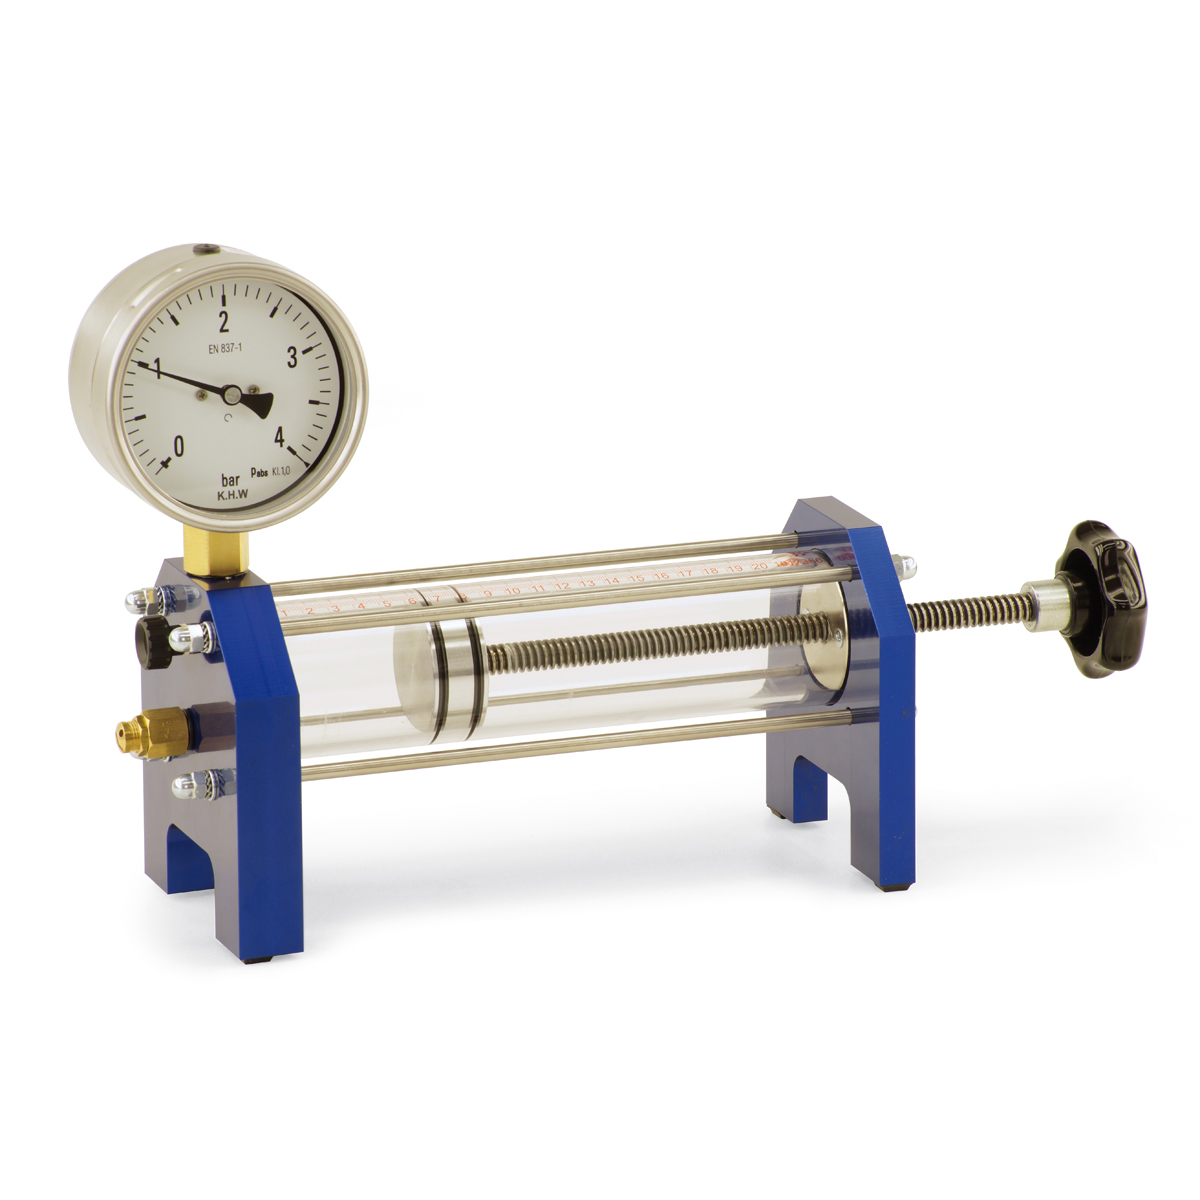
\includegraphics[width = 0.3\textwidth]{image/image2.png}
    
    \caption{Установка для демонстации закона Бойля-Мариотта}
    
    \label{fig:установка для демнострации закона Бойля-Мариотта}
\end{figure}

\textbf{Ход работы:}

\begin{enumerate}
    \item{Открыли запорный вентиль на левой опоре установки.}
    \item{Установили поршень внутри прозрачноо цилиндра в положение \texttt{$S_0$} = 20 см и закрыли вентиль.}
    \item{Сняли показание давления и записли в таблицу 1.}
    \item{Изменяли положение поршня по 1"=му см. В каждом положении снимали и записывали показания давления в цилиндре}
    \item{Установили поршень в положение \texttt{$S_0$}, открыли вентиль, сбросив давление, и закрыли.}
    \item{Затем установили поршень в положение \texttt{$S$} = 20. Изменяли положение поршня пошагово по 1"=му см. В каждом положении снимали и регистрировали показания давления.}
    \item{Установили поршень в положение \texttt{$S_0$} = 5, открыли вентиль сбросив давление, и закрыли.}
    \item{Затем установили поршень в положение \texttt{$S$} = 20. Изменяли положение поршня пошагово по 1"=му см. В каждом положении давления.}
    \item{Расчитали объем воздуха \texttt{$V$}, находящегося в закрытом пространстве цилиндра лаборатоной установки по данным о расстоянии \texttt{$S$}, на котором находится поршень по отношению к положению нулевого объема и площади поперечного сечения A поршня.}
    \item{Рассчитали при помощи уравнения \texttt{$p V = \nu R T$}, (где \texttt{$T$} "--- температура газа, \texttt{$R$} "--- универсальная газовая постоянная, \texttt{$\nu$} "--- количество вещества) количество вещества в цилиндре, выраженное в молях}
    
    $
        \nu_1 = \frac{565.49}{8.314 \cdot 293.15} \approx 23.2 \text{мМоль}
    $
    
    $
        \nu_2 \approx 46.4 \text{мМоль}
    $
    
    $
        \nu_3 \approx 92.81 \text{мМоль}
    $
    \item{Построили графики зависимости $P$ от $V$ (рис.\ref{graph:main_graph})}
\end{enumerate}

\textbf{Эксперементальные данные:}

Эксперементальные данные представленны в таблице \ref{tab:main_tab}
\begin{table}[H]
    \centering
    \begin{tabular}{|c|c|c|c|c|}
        \hline
        \makecell{Положение \\ поршня \texttt{$S$}, см} & 
        \makecell{Рабочий объем \\ цилиндра \texttt{$V$},см$^3$} &
        \multicolumn{3}{|c|}{\makecell{Давление воздуха при различном \\ его количестве в рабочем объеме \\ цилиндра \texttt{$p$}, бар}} \\
        \cline{3-5}
        & & \texttt{$S_0 = 20$} & \texttt{$S_0 = 10$} & \texttt{$S_0 = 5$}\\ 
        \hline 
        1 & 113.09 & - & - & 3 \\
        \hline 
        2 & 226.19 & - & 3.84 & 2.12 \\
        \hline 
        3 & 339.29 & - & 2.9 & 1.55 \\
        \hline 
        4 & 452.39 & - & 2.29 & 1.22 \\
        \hline 
        5 & 565.49 & 3.63 & 1.9 & 1 \\
        \hline 
        6 & 678.58 & 3.09 & 1.61 & 0.85 \\
        \hline 
        7 & 791.68 & 2.7 & 1.4 & 0.73 \\
        \hline 
        8 & 904.78 & 2.4 & 1.23 & 0.65 \\
        \hline 
        9 & 1017.9 & 2.15 & 1.1 & 0.58 \\
        \hline 
        10 & 1130.97 & 1.95 & 1 & 0.5 \\
        \hline 
        11 & 1244.1 & 1.79 & 0.91 & 0.47 \\
        \hline 
        12 & 1357.2 & 1.64 & 0.84 & 0.43 \\
        \hline 
        13 & 1470.3 & 1.51 & 0.78 & 0.4 \\
        \hline 
        14 & 1583.4 & 1.4 & 0.71 & 0.36 \\
        \hline 
        15 & 1696.5 & 1.31 & 0.67 & 0.35 \\
        \hline 
        16 & 1809.6 & 1.22 & 0.62 & 0.33 \\
        \hline 
        17 & 1922.7 & 1.18 & 0.59 & 0.3 \\
        \hline 
        18 & 2035.8 & 1.1 & 0.55 & 0.28 \\
        \hline 
        19 & 2148.8 & 1.05 & 0.52 & 0.26 \\
        \hline 
        20 & 2261.9 & 1 & 0.5 & 0.25 \\
        \hline
\end{tabular}
\caption{Эксперементальныйе данные}
\label{tab:main_tab}
\end{table}

Вывод:

В лабораторной работе мы проверили закон Бойля"=Мариотта, измерили давление воздуха при постоянном количестве вещества и температуре, передвигая поршень, и построили графики зависимости давления от объёма. Закон Бойля"=Мариотта действует, т.к. для всех измеренных значений \texttt{$p V = const$} построенные графики гиперболические, что так же подтверждает закон

\begin{figure}[!h]
\begin{center}
\begin{tikzpicture}
    \begin{axis}
        [
            width=\linewidth, % Scale the plot to \linewidth 
            legend pos = north east,
            xlabel=$V ~ \text{см}^3$, % Set the labels
            ylabel=$p ~ \text{бар}$,
            ymin = 0,
            xmin = 0,
            grid = major
        ]
        \addplot table[x=column 1,y=column 2,col sep=comma] {csvTable/table1.csv}; 
        \addplot table[x=column 1,y=column 2,col sep=comma] {csvTable/table2.csv};
        \addplot table[x=column 1,y=column 2,col sep=comma] {csvTable/table3.csv};
        \legend{
            \texttt{$S_0 = 20$},
            \texttt{$S_0 = 10$},
            \texttt{$S_0 = 5$},
        };
      \end{axis}
    \end{tikzpicture}
  \end{center}
\caption{График зависимости \texttt{$P$} от \texttt{$V$}}
\label{graph:main_graph}
\end{figure}



\section{Бальшой длинный формулы))))))}
\texttt{$\gamma$}  "--- отношение теплоемкостей

\texttt{$m$} "--- масса газа

начальные состояния:

\begin{enumerate}
    \item {$V_0$ "--- объем}
    \item {$p_0$ + $H$ "--- давление, где ($p_0$ "--- атмосферное давление, $H$ "--- разность уровней жидкости в манометре) }
    \item {$T_0$ "--- температура}
\end{enumerate}

состояние в конце процесса:

\begin{enumerate}
    \item {$V_1$ "---  объем}
    \item {$p_0$ + $H'$ "--- давление, где ($p_0$ "--- атмосферное давление, $H'$ "--- разность уровней жидкости в манометре) }
    \item {$T_1$ "--- температура}
\end{enumerate}

\begin{equation}
    \label{eq : second_eq}
    p_0 \cdot V_0^\gamma = (p_0 + H)V_0^\gamma
\end{equation}
\begin{equation}
    \label{eq : third_eq}
    (p_0 + H) \cdot V_0 = (p_0 + H')V_1
\end{equation}

из \ref{eq : second_eq} и \ref{eq : third_eq}

\begin{equation*}
    (\frac{V_0}{V_1})^\gamma = \frac{p_0}{p_0 + H} 
\end{equation*}

\begin{equation*}
    (\frac{V_0}{V_1})^\gamma = \frac{(p_0 + H')^\gamma }{(p_0 + H)^\gamma}
\end{equation*}

откуда 

\begin{equation*}
    \frac{p_0}{p_0 + H}  = \frac{(p_0 + H')^\gamma }{(p_0 + H)^\gamma}
\end{equation*}

Логарифмируя это выражение, получим:

\begin{equation*}
    ln \frac{p_0}{p_0 + H}  = \gamma ln \frac{(p_0 + H')}{(p_0 + H)}
\end{equation*}

Определим отсюда:

\begin{equation*}
    \gamma = \frac{ln \frac{p_0}{p_0 + H}}{ln \frac{(p_0 + H')}{(p_0 + H)}} = \frac{ln (1 - \frac{H}{p_0 + H})}{ln(1- \frac{(H - H')}{(p_0 + H)})}
\end{equation*}

разлагая логарифмы в ряды по формуле:

\begin{equation*}
    ln (1-x)  = -x + \frac{1}{2} x^2 -\frac{1}{3} x^3 +....
\end{equation*}

и ограничиваясь только первыми членами разложения, найдем приближенно:

\begin{equation*}
    \gamma = \frac{- \frac{H}{p_0 + H}}{- \frac{(H - H')}{(p_0 + H)}} = \frac{H}{H-H'}
\end{equation*}


\section{Код на c++ с использованием minted}
\inputminted[]{c++}{c++_file/task_gallows.cpp}


\bibliographystyle{ugost2003}
\bibliography{thesis}



\end{document}